%preamble - package inclusion and set up
\documentclass[10pt,twoside,a4paper,english]{report} %normalt 12pt!!!!
% Select encoding of your inputs
\usepackage[utf8]{inputenc}

% Make latex understand and use the typographic
% rules of the language used in the document.
%\usepackage[danish]{babel}
\usepackage[english]{babel}

% Use the vector font Latin Modern which is going
% to be the default font in latex in the future.
\usepackage{lmodern}

% Choose the font encoding
\usepackage[T1]{fontenc}

% Use color in tables
\usepackage[table]{xcolor}
\usepackage{pbox}
\usepackage{tabularx}
\usepackage{array}
\usepackage{multirow}

% Load a colour package
\usepackage{xcolor}
\definecolor{aaublue}{RGB}{33,26,82}  %<--define aaublue
\definecolor{white}{RGB}{255,255,255} %<--define white

% ref stuffz
\usepackage{cleveref}

% The standard graphics inclusion package
\usepackage{graphicx}

\makeatletter
  \g@addto@macro\@floatboxreset\centering %<--centering all figures
\makeatother

\usepackage{adjustbox}

% Set up how figure and table captions are displayed

\usepackage{float}
\restylefloat{figure}
\usepackage{caption}
\usepackage{subfigure}
\captionsetup
{
  justification = centering,    %<--centering caption with multiple lines
  font          = footnotesize, %<--set font size to footnotesize
  labelfont     = bf            %<--bold label (e.g., Figure 3.2) font
}
\captionsetup[subfigure]
{
  justification = centering, %<--centering subfigure caption text
  singlelinecheck=false,
  font = footnotesize        %<--font size for subfigures
} 

% Enable row combination in tables
\usepackage{multirow}

% Make space between table lines and text
\renewcommand{\arraystretch}{1.5}

% Enable commands like \st (strike out) and \hl (high light)
\usepackage{soul}

% Make the standard latex tables look so much better
\usepackage{array,booktabs}

% Enable the use of frames around, e.g., theorems
% The framed package is used in the example environment
\usepackage{framed}
\usepackage{colortbl}
\usepackage{longtable}
\usepackage{xcolor}
\usepackage{textcomp}

%-------MATHEMATICS---------------------------------
% Defines new environments such as equation,
% align and split 
\usepackage{amsmath}
\usepackage{relsize}
% Adds new math symbols
\usepackage{amssymb}
% Use theorems in your document
% The ntheorem package is also used for the example environment
% When using thmmarks, amsmath must be an option as well. Otherwise \eqref doesn't work anymore.
\usepackage[framed,amsmath,thmmarks]{ntheorem}
\usepackage{xifthen}%<--enables ifthenelse which is used in macros

\usepackage{siunitx} 
\sisetup{decimalsymbol=period}%<--\num{} will swich commas with periods
\sisetup{detect-weight}
%---------------------------------------------------

%-------PAGE LAYOUT---------------------------------
% Change margins, papersize, etc of the document
\usepackage[
  left=25mm,% left margin on an odd page %tidligere 25mm for baade right og left
  right=25mm,% right margin on an odd page
  top=35mm,
  ]{geometry}
  
% Modify how \chapter, \section, etc. look
% The titlesec package is very configureable
\usepackage{titlesec}
\makeatletter
\def\ttl@mkchap@i#1#2#3#4#5#6#7{%
    \ttl@assign\@tempskipa#3\relax\beforetitleunit
    \vspace{\@tempskipa}%<<<<<< REMOVE THE * AFTER \vspace
    \global\@afterindenttrue
    \ifcase#5 \global\@afterindentfalse\fi
    \ttl@assign\@tempskipb#4\relax\aftertitleunit
    \ttl@topmode{\@tempskipb}{%
        \ttl@select{#6}{#1}{#2}{#7}}%
    \ttl@finmarks  % Outside the box!
    \@ifundefined{ttlp@#6}{}{\ttlp@write{#6}}}
\makeatother

\titlespacing{\chapter}{0pt}{0pt}{10pt}
\titlespacing{\section}{0pt}{0pt}{-5pt}
\titlespacing{\subsection}{0pt}{8pt}{-5pt}
\titlespacing{\subsubsection}{0pt}{6pt}{-10pt}

\titleformat*{\section}{\normalfont\Large\bfseries\color{aaublue}}
\titleformat*{\subsection}{\normalfont\large\bfseries\color{aaublue}}
\titleformat*{\subsubsection}{\normalfont\normalsize\bfseries\color{aaublue}}

\usepackage{titlesec, blindtext, color}
%\color{gray75}{gray}{0.75}
\newcommand{\hsp}{\hspace{20pt}}
\titleformat{\chapter}[hang]{\Huge\bfseries}{\thechapter\hsp\textcolor{aaublue}{|}\hsp}{0pt}{\Huge\bfseries}

% Change the headers and footers
\usepackage{fancyhdr}
\setlength{\headheight}{15pt}
\pagestyle{fancy}
\fancyhf{} %delete everything
\renewcommand{\headrulewidth}{0pt} %remove the horizontal line in the header
\fancyhead[RO,LE]{\color{aaublue}\small\nouppercase\leftmark} %even page - chapter title
\fancyhead[LO]{}
\fancyhead[RE]{} 
\fancyhead[CE]{}
\fancyhead[CO]{}
\fancyfoot[RE,LO]{\thepage}
\fancyfoot[LE,RO]{} %page number on all pages
\fancyfoot[CE,CO]{}

% change first page of all chapters header and footer to fancy style
\makeatletter
\let\ps@plain\ps@fancy
\makeatother

% Do not stretch the content of a page. Instead,
% insert white space at the bottom of the page
\raggedbottom

% Enable arithmetics with length. Useful when typesetting the layout.
\usepackage{calc}
%---------------------------------------------------

\usepackage{appendix}

%-------BIBLIOGRAPHY--------------------------------
%setting references (using numbers) and supporting i.a. Chicargo-style:
\usepackage{etex}
\usepackage{etoolbox}
\usepackage{keyval}
\usepackage{ifthen}
\usepackage{url}
\usepackage{csquotes}
\usepackage[backend=biber, url=true, doi=true, style=numeric, sorting=none]{biblatex}
\addbibresource{setup/bibliography.bib}
%---------------------------------------------------

%-------MISC----------------------------------------
%%% Enables the use FiXme refferences. Syntax: \fxnote{...} %%%
\usepackage[footnote, draft, english, silent, nomargin]{fixme}		%!!!! DRAFT OR FINAL?!?!?!?!11!! change later!	
%With "final" instead of "draft" an error will ocure for every FiXme under compilation.

%%% allows use of lorem ipsum (generate i.e. pagagraph 1 to 5 with \lipsum[1-5]) %%%
\usepackage{lipsum}

%%% Enables figures with text wrapped tightly around it %%%
\usepackage{wrapfig}

%%% Section debth included in table of contents (1 = down to sections) %%%
\setcounter{tocdepth}{1}

%%% Section debth for numbers (1 = down to sections) %%%
\setcounter{secnumdepth}{2}

\usepackage{tocloft}
\setlength{\cftbeforetoctitleskip}{0 cm}
\renewcommand{\cftpartpresnum}{Del~}
\let\cftoldpartfont\cftpartfont
\renewcommand{\cftpartfont}{\cftoldpartfont\cftpartpresnum}
%---------------------------------------------------

%-------DANSK SPROG---------------------------------

%\addto\captionsdanish{%
%	\renewcommand{\figurename}{figur}%
%	\let\figureautorefname\figurename%
%	\renewcommand{\tablename}{tabel}%
%	\let\tableautorefname\tablename%
%%	\renewcommand{\equationname}{ligning}%
%%	\let\equationautorefname\equationname%
%	\renewcommand{\chaptername}{Kapitel}%
%	\let\chapterautorefname\chaptername%
%	\renewcommand{\partname}{Del}%
%	\let\partautorefname\partname%
%	\renewcommand{\sectionname}{afsnit}%
%	\let\sectionautorefname\sectionname%
%%	\renewcommand{\thesubsection}{underafsnit}%
%%	\let\subsectionautorefname\thesubsection%
%	\renewcommand{\pagename}{side}%
%	\let\pageautorefname\pagename%
%}

%-------HYPERLINKS----------------------------------
% Enable hyperlinks and insert info into the pdf
% file. Hypperref should be loaded as one of the 
% last packages
\usepackage{nameref}
\usepackage{hyperref}
\usepackage{bookmark}
\hypersetup{%
	%pdfpagelabels=true,%
	plainpages=false,%
	pdfauthor={Author(s)},%
	pdftitle={Title},%
	pdfsubject={Subject},%
	bookmarksnumbered=true,%
	colorlinks,%
	citecolor=aaublue,%
	filecolor=aaublue,%
	linkcolor=aaublue,% you should probably change this to black before printing
	urlcolor=aaublue,%
	pdfstartview=FitH%
}

\crefname{appsec}{bilag}{bilag}
%---------------------------------------------------

% remove all indentations
\setlength\parindent{0pt}
\parskip 5mm
\usepackage{verbatim}

\definecolor{Gra}{RGB}{230,230,230}

%creates a nice-looking C#-text
\newcommand{\CC}{C\nolinebreak\hspace{-.05em}\raisebox{.3ex}{\scriptsize\text \#} }

%enables multi column lists
\usepackage{multicol}

%enables code-examples
\usepackage{listings}

\definecolor{coolblue}{RGB}{32,95,128}
\definecolor{mygreen}{rgb}{0,0.6,0}
\definecolor{mygray}{rgb}{0.5,0.5,0.5}
\definecolor{mymauve}{rgb}{0.58,0,0.82}
\usepackage{textcomp}
\definecolor{listinggray}{gray}{0.9}
\definecolor{lbcolor}{rgb}{0.9,0.9,0.9}

%for c code
\lstdefinestyle{cstyle}{
  backgroundcolor=\color{lbcolor},
	tabsize=4,
	rulecolor=,
	language=C,
  basicstyle=\scriptsize,
  upquote=true,
  aboveskip={1.5\baselineskip},
  columns=fixed,
  showstringspaces=false,
  extendedchars=true,
  breaklines=true,
  prebreak = \raisebox{0ex}[0ex][0ex]{\ensuremath{\hookleftarrow}},
  frame=single,
  showtabs=false,
  numbers=left,
  captionpos=b,
  numbersep=5pt,
  numberstyle=\tiny\color{mygray},
  showspaces=false,
  showstringspaces=false,
  identifierstyle=\ttfamily,
  keywordstyle=\color[rgb]{0,0,1},
  commentstyle=\color[rgb]{0.133,0.545,0.133},
  stringstyle=\color[rgb]{0.627,0.126,0.941},
}
%for python code
\lstdefinestyle{pythonstyle}{
    backgroundcolor=\color{lbcolor},
    tabsize=4,
    rulecolor=,
    language=python,
    basicstyle=\scriptsize,
    upquote=true,
    aboveskip={1.5\baselineskip},
    columns=fixed,
    showstringspaces=false,
    extendedchars=true,
    breaklines=true,
    prebreak = \raisebox{0ex}[0ex][0ex]{\ensuremath{\hookleftarrow}},
    frame=single,
    showtabs=false,
    numbers=left,
    captionpos=b,
    numbersep=5pt,
    numberstyle=\tiny\color{mygray},
    showspaces=false,
    showstringspaces=false,
    identifierstyle=\ttfamily,
    keywordstyle=\color[rgb]{0,0,1},
    commentstyle=\color[rgb]{0.133,0.545,0.133},
    stringstyle=\color[rgb]{0.627,0.126,0.941},
}
%for matlab code
\lstdefinestyle{matlabstyle}{
    backgroundcolor=\color{lbcolor},
    tabsize=4,
    rulecolor=,
    language=Matlab,
    basicstyle=\scriptsize,
    upquote=true,
    aboveskip={1.5\baselineskip},
    columns=fixed,
    showstringspaces=false,
    extendedchars=true,
    breaklines=true,
    prebreak = \raisebox{0ex}[0ex][0ex]{\ensuremath{\hookleftarrow}},
    frame=single,
    showtabs=false,
    numbers=left,
    captionpos=b,
    numbersep=5pt,
    numberstyle=\tiny\color{mygray},
    showspaces=false,
    showstringspaces=false,
    identifierstyle=\ttfamily,
    keywordstyle=\color[rgb]{0,0,1},
    commentstyle=\color[rgb]{0.133,0.545,0.133},
    stringstyle=\color[rgb]{0.627,0.126,0.941},   
}

%for java code
\lstdefinestyle{javastyle}{
	backgroundcolor=\color{lbcolor},
	tabsize=4,
	rulecolor=,
	language=Java,
	basicstyle=\scriptsize,
	upquote=true,
	aboveskip={1.5\baselineskip},
	columns=fixed,
	showstringspaces=false,
	extendedchars=true,
	breaklines=true,
	prebreak = \raisebox{0ex}[0ex][0ex]{\ensuremath{\hookleftarrow}},
	frame=single,
	showtabs=false,
	numbers=left,
	captionpos=b,
	numbersep=5pt,
	numberstyle=\tiny\color{mygray},
	showspaces=false,
	showstringspaces=false,
	identifierstyle=\ttfamily,
	keywordstyle=\color[rgb]{0,0,1},
	commentstyle=\color[rgb]{0.133,0.545,0.133},
	stringstyle=\color[rgb]{0.627,0.126,0.941},
}

%for inline c, syntax: \cline{ codeHere(); }
\lstdefinestyle{cinline}{
    style=cstyle,
    basicstyle=\small,
}
\newcommand\inlinec[1]{ \lstinline[style=cinline]{#1} }

%for inline python, syntax: \pythonline{ codeHere(); }
\lstdefinestyle{pythoninline}{
    style=pythonstyle,
    basicstyle=\small,
}
\newcommand\inlinepython[1]{ \lstinline[style=pythoninline]{#1} }

%for inline matlab, syntax: \matlabline{ codeHere(); }
\lstdefinestyle{matlabinline}{
    style=matlabstyle,
    basicstyle=\small,
}
\newcommand\inlinematlab[1]{ \lstinline[style=matlabinline]{#1} }

\usepackage{enumitem}
%\usepackage[citestyle=authoryear,natbib=true]{biblatex}

% Figures - TIKZ
\usepackage{tikz}
\usepackage[americanresistors,americaninductors,americancurrents, americanvoltages]{circuitikz}

% Wall of text logo
\newcommand{\walloftextalert}[0]{\includegraphics[width=\textwidth]{walloftext.png}}

\usepackage{pdfpages}
\usepackage{lastpage}
\usepackage{epstopdf}

\setlength{\headheight}{21pt}

\hfuzz=\maxdimen
\tolerance = 10000
\hbadness  = 10000

\usepackage{siunitx}
\graphicspath{{./figures/}}

%macros - please read this file
%Macro for 'where'-enviroment was improved by Andrea and Niels :-)

%-----------UNITS-------------------------------------------
\newcommand{\unit}[1]{&& \left[\si{#1}\right]}
%
%\newcommand{\unit}[1]{[\si{#1}]}            %<<| Use these if you want equations to be
%\newcommand{\eq}[2]{&&\si{#1} &= \si{#2}&&} %<<| centered.. .. will appear scrambled
%                                            %  | from one equation to the next though..
%                                            %  | and does not work with long equations.. :/
%
%-----------------------------------------------------------

%-----------WHERE ENVIRONMENT-------------------------------
\newenvironment{where}{\leavevmode{\parindent=1em\indent} Where:\\}{}
\newcommand{\va}[3]
{
  \begin{tabular}{p{20pt} p{40pt} p{290pt} l}
    & { $#1$ } & { #2 } & \ifthenelse{\isempty{ #3 }}  {}  {[{\si{#3}}]} \\
  \end{tabular}\\
}
%-----------------------------------------------------------

%-----------TikZ SETTINGS-----------------------------------
\tikzset{
  block/.style    = {draw, thick, rectangle,
                     minimum height = 2.1em,
                     minimum width = 1.7em},
  sum/.style      = {draw, circle, inner sep=3pt} %<--Adder
}
%-----------------------------------------------------------


%-----------Fanzy reference SETTINGS------------------------
%Figure references:
\newcommand{\figref}[1]{figure \ref{#1}}

%Figure references after full stop/period:
\newcommand{\Figref}[1]{Figure \ref{#1}}

%Table references:
\newcommand{\tabref}[1]{table \ref{#1}}

%Table references after full stop/period:
\newcommand{\Tabref}[1]{Table \ref{#1}}

%Section references:
\newcommand{\secref}[1]{section \ref{#1} on site \pageref{#1}}

%Section references:
\newcommand{\Secref}[1]{Section \ref{#1} on site \pageref{#1}}

%Appendix references:
\newcommand{\appref}[1]{appendix \ref{#1} on site \pageref{#1}}

%Appendix references:
\newcommand{\Appref}[1]{Appendix \ref{#1} on site \pageref{#1}}

%chapter references: 
\newcommand{\chapref}[1]{chapter \ref{#1} on site \pageref{#1}}

%chapter references: 
\newcommand{\Chapref}[1]{Chapter \ref{#1} on site \pageref{#1}}

%Units:
%\newcommand{\unit}[1]{&& \left[\si{#1}\right]}

%Text:
\newcommand{\tx}[1]{\text{#1}}

%Equation references:
%1 equation:
\renewcommand{\eqref}[1]{equation (\ref{#1})}

%-----------------------------------------------------------





\begin{document}       % TIP: If you are using TeXstudio you can open
%\tableofcontents      %      the file by Ctrl+LeftClick on setup/macros.tex
\pagebreak             %      If the file doesn't exist, you will be asked
					   %      weather or not you want to create it.


%||||||||||||||||||||||||||||||||||||||||||||||||||||||||||||||||
%|||||||                 Example Inputs                  ||||||||
%||||||||||||||||||||||||||||||||||||||||||||||||||||||||||||||||
%|||||||                                                 ||||||||
%			 \chapter{Figure Sample}

\begin{figure}[H]                                         %   File-type can be specified
  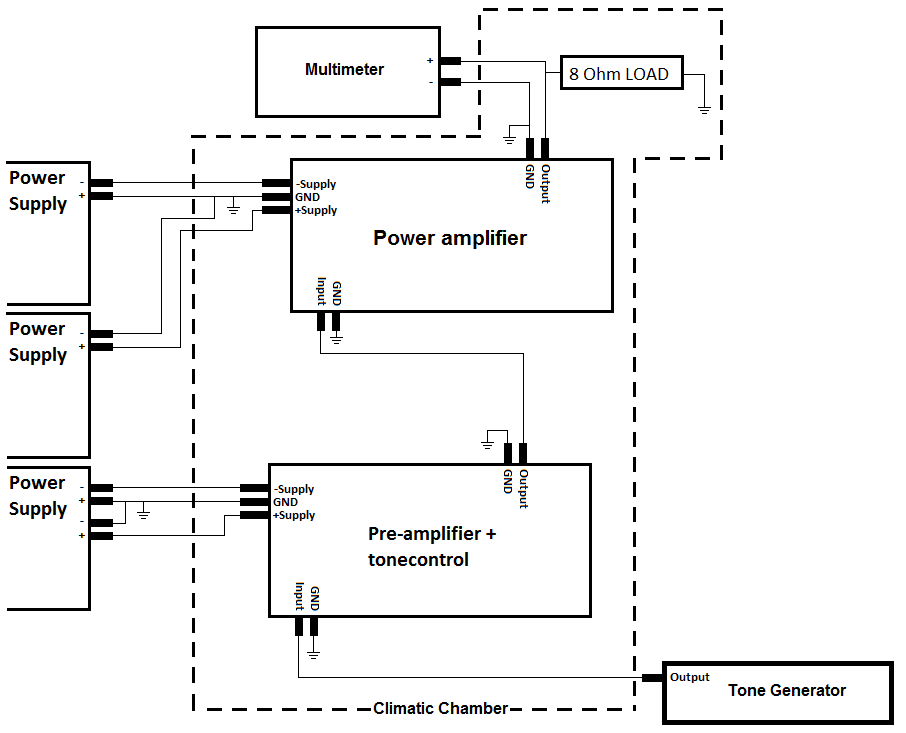
\includegraphics[width=.4\textwidth]{figures/filename}  %<--but is not needed.
  \caption{This image is clearly too small, remember to scale appropriately \fxnote{Remember source}}
  \label{fig:FigureLABEL}  %<--give the figure a label, so you can reference!
\end{figure}               %   For the label to work it must be under the caption.

% Fxnotes will not compile properly inside the figure, only in the caption.
% When \fxnote{} is used in caption, it does not show in a footnote as it normally 
% would, it does however appear in list of corrections.

\autoref{fig:FigureLABEL} $\leftarrow$ use autoref, unless you are referring to multiple pictures, then do like this: \autoref{fig:HbridgeClokwise4Q} and \ref{fig:HbridgeCounterClokwise4Q}.

%Do NOT use \vspace{length}, \hspace{length} or \noindent etc. unless exceedingly necessary - LaTeX is a markup language, let it do its job.
\vspace{.5cm}
\noindent
%
%--------- BIBLIOGRAPHY REF EKSAMPLE -----------------------------------
This reference only represents this line since it is before the punctuation mark\cite{YDing}. This next reference however represents the entire section. That is, all of the preceding sentences in the entire section. This is due to the fact that it is now after the punctuation mark in the end of the section (this is not used in the middle of a section!).\cite{YDing}

%>>PLEASE ALSO READ THE NOTE IN bibliography/bibliography.bib<<

Here is a way to make two images appear on the side of each other. Also, if you modified an image, this is how you properly refer to its original source:

\begin{figure}[H]
    \subcaptionbox  %<--use captionbox instead if no global caption is needed
    {               %                                \%-%-%-%-%-%-%\
      Clockwise 4Q operation.\newline                              %\
      \emph{Edited from image by Biezl.\cite{Biezl}}                %\
      \label{fig:HbridgeClokwise4Q}                                  %\
    }                                                                 %\
    {                                                                  %\
      \includegraphics[width=.46\textwidth]{HbridgeClockwise4Q}         %\
    }                                                                    %\
    \hspace{5pt}                                                          %\
    \subcaptionbox  %<-----------------------------------------------------%\
    {                                                                       %\
      Counterclockwise 4Q operation.\newline                                 %\
      \emph{Edited from image by Biezl.\cite{Biezl}}                          %\
      \label{fig:HbridgeCounterClokwise4Q}                                     %\
    }                                                                           %\
    {                                                                            %\
      \includegraphics[width=.46\textwidth]{HbridgeCounterClockwise4Q}            %|
    }                                                                             %|
    \caption{The 4 quadrant H-bridge configuration shown in both directions.}%<-%-/
    \label{fig:Hbridges}
\end{figure}

As seen \autoref{fig:HbridgeCounterClokwise4Q} can be referred to on its own, or you can use \autoref{fig:Hbridges} to refer to both \autoref{fig:HbridgeClokwise4Q} and \autoref{fig:HbridgeCounterClokwise4Q}.

If the figures are not directly related you might not want to use \textbf{(a)} and \textbf{(b)}, but instead give each figure their own label, here is an example:

\begin{figure}[H]
    \captionbox
    {
      Clockwise 4Q operation.\newline
      \emph{Edited from image by Biezl.\cite{Biezl}}
      \label{fig:HbridgeClokwise4Q2}
    }
    {
      \includegraphics[width=.46\textwidth]{HbridgeClockwise4Q}
    }
    \hspace{5pt}
    \captionbox
    {
      Counterclockwise 4Q operation.\newline
      \emph{Edited from image by Biezl.\cite{Biezl}}
      \label{fig:HbridgeCounterClokwise4Q2}
    }
    {
      \includegraphics[width=.46\textwidth]{HbridgeCounterClockwise4Q}
    }
\end{figure}

In this case \autoref{fig:HbridgeClokwise4Q2} can be referred to without involving \autoref{fig:HbridgeCounterClokwise4Q2}.

\pagebreak			 %|||||||
%			 \section{Table Sample} %to view this sample properly in the code, the screen must be
                       %wide enough, or you have to disable word-wrap in your editor.
\begin{table}[H]
\begin{tabular}{|l|p{5cm}|l|l|l|}
  \hline %-----------------------------------------------------------------------------------
  \textbf{No.} &\textbf{Description} &\textbf{Min} &\textbf{Max} &\textbf{Requirements}    \\
  \hline %-----------------------------------------------------------------------------------
  1            & Some Text           & Some Text   & Some Text   & Some Text               \\
               &                     &             &             & Some More Text          \\
               &                     &             &             & Text Text               \\
               &                     &             &             & Text Text Text          \\
  \hline %-----------------------------------------------------------------------------------
  2            & Some Text           & Some Text   & Some Text   & Some Text               \\
  \hline %-----------------------------------------------------------------------------------
  3            & By specifying the
                 width of a column
                 (|p\{5cm\}|) the
                 cells in that column
                 will not exceed the
                 specified width but         %Extra whitespace is used only for clarity
                 instead expand              %and will not affect the compiled output.
                 downward.
                                     & Some Text           & Some Text   & Some Text       \\
  \hline %-----------------------------------------------------------------------------------
  4            & Some Text           & Some Text   & Some Text   & Some Text               \\
  \hline %-----------------------------------------------------------------------------------
  \multicolumn{2}{|l|}{Some Text}    & \multicolumn{3}{l|}{Some Text}                      \\
  \hline %-----------------------------------------------------------------------------------
  \multicolumn{2}{|l|}{Text Text}    & \multicolumn{3}{l|}{Text = Text}                    \\
  \multicolumn{2}{|l|}{}             & \multicolumn{3}{l|}{Text = Text}                    \\
  \multicolumn{2}{|l|}{}             & \multicolumn{3}{l|}{Text = Text}                    \\
  \multicolumn{2}{|l|}{}             & \multicolumn{3}{l|}{Text = Text}                    \\
  \multicolumn{2}{|l|}{}             & \multicolumn{3}{l|}{Text = Text}                    \\
  \hline %-----------------------------------------------------------------------------------
  \multicolumn{2}{|l|}{Some Text}    & \multicolumn{3}{l|}{Teeeexxtt}                      \\
  \multicolumn{2}{|l|}{}             & \multicolumn{3}{l|}{\LaTeX}                         \\
  \hline %-----------------------------------------------------------------------------------
\end{tabular}
\caption{This Is a Table\label{table:TableLABEL}}
\end{table}

\autoref{table:TableLABEL} $\leftarrow$ use autoref, unless you are referring to multiple tables, then do like this: \autoref{table:TableLABEL} and \ref{table:TableLABEL}.

\pagebreak 		     %|||||||
%			 \section{Equation Sample} %<--In American English all Important Words in
                          %   Headlines are with Big Letters

% \unit is a macro. It uses SI units and aligns all the units neatly :)

\textbf{A normal equation:}
\begin{flalign}
  J_m \cdot \dot{\omega}_m(t) &= \tau_m(t) - B_m \cdot \omega_m(t) - r_m \cdot f_c(t)& \unit{N \cdot m}
  \label{eq:MotorGearNewtonSecLaw}
\end{flalign}
%
\begin{where}
  \va{ J_m               }{is the motor's inertia}                     {kg \cdot m^2}
  \va{ \omega_m(t)       }{is the angular velocity of the motor}       {rad \cdot s^{-1}}
  \va{ \dot{\omega}_m(t) }{is the angular acceleration of the motor}   {rad \cdot s^{-2}}
  \va{ \tau_m(t)         }{is the torque delivered by the motor}       {N \cdot m}
  \va{ B_m               }{is the motor's friction coefficient}        {N \cdot m \cdot s \cdot rad^{-1}}
  \va{ r_m               }{is the radius of the gear, $G_m$}           {m}
  \va{ f_c(t)            }{is the contact force between the two gears} {N}
\end{where}

\textbf{If you need to write something with numbers:} %<--Do not use \textbf{} as headlines, it is bad practice
                                                      %   use instead \chapter{}, \section{}, \subcaption{}, \subsubsection{}
                                                      %   in that order - never a \subsubsection{} directly under a \section{}
\begin{flalign}
  B      &= \num{2,2}\cdot 10^{-6}  \ \si{N\cdot m \cdot rad^{-1} \cdot s}& \label{eq:eq2} \\ %<-- if you want two equations to
  \tau_c &= \num{0.0016}            \ \si{N\cdot m}                       & \label{eq:eq3}    %    allign in one envirenment,
\end{flalign}                                                                              %    remember \\
%using \num{} ensures the same use of decimal point throughout the repport
%should you want to change it, the option is set in the preamble, just change 'period' to 'comma':
%\sisetup{decimalsymbol=period}

\autoref{eq:MotorGearNewtonSecLaw} $\leftarrow$ use autoref, unless you are referring to multiple equations, then do like this: \autoref{eq:eq2} and \ref{eq:eq3}.

\pagebreak		 %|||||||
%			 \section{TikZ Sample}

\textbf{TikZ is only for very patient people, I can recommend Inkscape with textext plugin: \url{https://pav.iki.fi/software/textext/}, difficult to install easy to use, and, if used carefully, nice results.}

%heavily commented example
\input{chapters/tikz/TikZblockDiagramSample.tex}

%way to keep the drawing code in a seperate file
\begin{figure}[H]
	\input{chapters/tikz/smallBlockDiagram.tikz}
	\centering
	\caption{Block diagram}
\end{figure}

%TikZ can also be used for circuits
\input{chapters/tikz/TikZcircuitSample.tex}


\pagebreak            %|||||||
%			 \section{Code Sample}

\begin{lstlisting}[ style=cstyle,
                    caption={C Code}, 
                    label=lst:cExample ]
#include "functions.h"

// Constant matrices
const float L[3] = { -11.0, -12.0, -13.0 };
const float B1[4] = { 0.0, -0.2396, 0.0, 0.2396 };
const float B2[4] = { 0.2396, 0.0, -0.2396, 0.0 };
const float B3[4] = { 0.0377, -0.0377, 0.0377, -0.0377 };
\end{lstlisting}

In \autoref{lst:cExample} is some C-code, and here is some in-line C-code: \inlinec{xTaskCreate();}.

\begin{lstlisting}[ style=pythonstyle,
                    caption={Python Code}, 
                    label=lst:pythonExample ]
# This parses the packets to identify messages and decodes them for the logs
class packetParser():
    def __init__(self,accelfile,gpsfile,measstate,fulllog,plog):
        self.GPS = {0: 'Latitude',
                    1: 'Longtitude',
                    2: 'Velocity'}
        self.IMU = {0: 'AccelerationX',
                    1: 'AccelerationY',
                    2: 'AccelerationZ',
                    3: 'GyroscopeX',
                    4: 'GyroscopeY',
                    5: 'GyroscopeZ',
                    6: 'MagnetometerX',
                    7: 'MagnetometerY',
                    8: 'MagnetometerZ',
                    9: 'Temperature'}
        self.MsgID = {0: self.GPS, 1: self.IMU}
        self.DevID = {0: 'GPS', 1: 'IMU'}
        self.accelburst = [0,0,0,0,0,0,0]
        self.accellog = accelfile
        self.fulllog = fulllog
\end{lstlisting}

In \autoref{lst:pythonExample} is some Python-code, and here is some in-line Python-code:\\ \inlinepython{self.plog.write(str(msgnr))}

\begin{lstlisting}[ style=matlabstyle,
                    caption={Matlab Code}, 
                    label=lst:matlabExample ]
  close all
  clear
  clc
  
  % Parameters
  mx=200;     % [kg] mass + added mass in xb direction
  my=250;     % [kg] mass + added mass in yb direction
  Iz=700;     % [kgm2]
  
  dx=70;      % [kg/s] 
  dy=100;     % [kg/s]
  dyaw=50;    % [kgm2/s]
\end{lstlisting}

In \autoref{lst:cExample}, \ref{lst:pythonExample} and \ref{lst:matlabExample} is some code, and here is some in-line matlab: \inlinematlab{randn(50)}            %|||||||
%|||||||                                                 ||||||||
%||||||||||||||||||||||||||||||||||||||||||||||||||||||||||||||||
%||||||||||||||||||||||||||||||||||||||||||||||||||||||||||||||||


%%% Prereport %%%
\setlength\cftaftertoctitleskip{2pt}
\setlength\cftafterloftitleskip{6pt}
\setlength\cftafterlottitleskip{6pt}
%\selectlanguage{danish}
\title{Simultaneous and proportional control of reaching and grasping}

%%% Frontmatter Settings %%%
\pagestyle{empty} %disable headers and footers
\pagenumbering{roman} %use roman page numbering in the frontmatter I II...
\fancyfoot[RE,LO]{17gr7404} %page number on all pages
\fancyfoot[LE,RO]{\thepage}
\fancyhead[LE,LO,RE,RO]{}

%%% Introductory Formalities %%%
%\includepdf[pages={1}]{formalities/frontpage.pdf}
\clearpage
\thispagestyle{empty}

\begin{figure}[H]
	\raggedleft
	
\includegraphics[width=0.2\textwidth]{figures/aaulogo-da.png}
\end{figure} 

\vspace{5 cm}

\begin{center}	
	\begin{Huge}
		\textbf{Simultaneous and proportional control of reaching and grasping}\\
		\vspace{5 mm}
		P$7$ Masterproject - Autumn $2017$\\
		\vspace{3 mm}
	\end{Huge}
	{\Large Gruppe $17$gr$7404$}
\end{center}
\vspace*{\fill}

\begin{center}
	\line(1,0){400}
\end{center}


\pagestyle{fancy}
%{\small
\strut\vfill % push the content to the bottom of the page
\noindent Copyright \copyright{} Aalborg University 2015\par
\vspace{0.2cm}

\noindent This report is compiled in \LaTeX, originally developed by Leslie Lamport, based on Donald Knuth's \TeX. The main text is written in \emph{Latin Modern} pt 12, designed by Bogusław Jackowski and Janusz M. Nowacki. 
%The document is compiled via the website \url{www.overleaf.com}, an online collaborative based \LaTeX-editor with instant preview, which enables multiple persons to edit the document simultaneously.
Flowcharts and diagrams are made using Microsoft Visio. 
\clearpage
%\begin{document} 
\thispagestyle{empty}
\begin{titlepage}
\begin{nopagebreak}
{\samepage 

\begin{tabular}{r}
\parbox{\textwidth}{  \raisebox{-15mm}{
\includegraphics[height=3cm]{figures/aaulogo-en.png}}
\hfill \hspace{2cm} \parbox{8cm}{\begin{tabular}{l} %4.90
{\small \textbf{\textcolor{aaublue}{{7\textsuperscript{th} Semester, Master Project}}}}\\
{\small \textbf{\textcolor{aaublue}{School of Medicine and Health}}}\\
%{\small \textbf{\textcolor{aaublue}{Communication Technologies}}}\\ 
{\small \textbf{\textcolor{aaublue}{Biomedical Engineering and Informatics}}}\\
{\small \textcolor{aaublue}{Fredrik Bajers Vej 7A}} \\
{\small \textcolor{aaublue}{9220 Aalborg}} \\
%{\small \textcolor{aaublue}{\emph{http://www.sict.aau.dk/electronics-and-it}}}
\end{tabular}}}
\end{tabular}

\begin{tabular}{cc}
\parbox{7cm}{

\textbf{Titel:}

title:\\ 

\textbf{Theme:}

\small{
Biomedical signals and information\\
}


\parbox{8cm}{


\textbf{Project period:}\\
P7, Autumn 2017\\
01/08/2017 - 19/12/2017\\
   
\textbf{Project group:}\\
17gr7404\\ %\fxnote{Input group number}
  
\textbf{Collaborators:}\\
Irene Uriarte \\
Martin Alexander Garenfeld \\
Oliver Thomsen Damsgaard \\
Simon Bruun \\

\textbf{Supervisors:}\\
Strahinja Dosen \\
Jakob Lund Dideriksen \\
Lotte N.S. Andreasen Struijk \\
}\\


\textbf{Pages:} 0\\
\textbf{Appendixes:} b \\
%\textbf{Ekstra:} For projektkode: Se forord\\ %eks. en CD eller USB
\textbf{Afsluttet:} 19/12/2017\\

\vfill } &
\parbox{7cm}{
  \vspace{.15cm}
  \hfill
  \begin{tabular}{l}
  {\textbf{Abstract}}\bigskip \\
  \fbox{
    \parbox{6.5cm}{\bigskip
     {\vfill{\small \lipsum[15]
%write real thing
     \bigskip}}
     }}
   \end{tabular}}
\end{tabular}} %\vspace{1cm}


\centering
\textit{Publication of this report's contents, including source references, may only happen in agreement with the authors.}\\
%\textit{Offentliggørelse af rapportens indhold, med kildeangivelse, må kun ske efter aftale med forfatterne.}\\


\end{nopagebreak}
\end{titlepage}
%\end{document} 			 % <--- this contains the synopsis!!
%%% Preface %%%
%\cleardoublepage
%\lipsum[15]
%write real thing
\clearpage
\chapter*{Preface}

\lipsum[9]

\pagebreak

\pdfbookmark[0]{Table of Contents}{label: tableOfCentents}
\tableofcontents
\cleardoublepage


%%% Mainmatter Settings %%%
\pagenumbering{arabic} %use arabic page numbering in the mainmatter
\fancyfoot[RO,LE]{\thepage \text{ of} \pageref{LastPage}}
\fancyfoot[RE,LO]{17gr7404}
\fancyhead[RE,LO]{}
\fancyhead[RE,LO]{\color{aaublue}\small\nouppercase\leftmark} %even page - chapter title
\pagestyle{fancy}


%---------------------------INPUTS-------------------------------
\chapter{Introduction}
% INTRO
%Introduction

%Why prostheses are important?
Upper limb prostheses have the purpose of fulfilling the users demand, which consists of cosmetic and functional support. The utmost wish for the consumer is to regain full appearance and function of the missing biological upper limb. The functionality is the most challenging aspects to fulfil. Two types of functional prostheses exist: body-powered and electrical, where the electrical has the highest functionality, and therefore ideally has a higher similarity to a biological upper limb. The most common electric prosthesis is the myoelectric prosthesis, where EMG signals are used as the control signal. \cite{jiang2012}. 
%What is an EMG-prosthesis?
%The performance of myoelctric prosthesis is based on the surface EMG signals adquisition from the muscles for further processing in order to activate different functions in the prosthesis

%What has been done in the EMG-prosthesis area?
In recent years the development of EMG controlled prosthetics have advanced considerably, due to an increased interest in the area along with a higher demand for better prosthetics and more precise control. \cite{Fougner2012} In the early years most EMG prosthetics functioned by only controlling one DOF by \textit{on-off control}, mostly by linking antagonistic muscles to one DOF. This kind of prostheses changes between states due a switching impulse which cause a state machine to shift its present state. Usually a strong and fast muscle contraction from the users are employ to generate the switching signals. \cite{amsuess2014}}
This type of control provided users a way to control more than one DOF, but never simultaneously. The switch-control functioned on a cycle, so users would have to go through all the movements of the prosthesis to find the one they wanted to perform. However, as demands would rise, more complex methods was introduced to the EMG scene. Classification methods effectively enabled users to use DOF's more freely because the switching was now replaced by direct recognition of different muscle contractions linked to specific prosthetic movements. This also effectively enabled proportional control of movements, but gave rise to new problems; a wider range of control would give less accurate movements, and training the classifiers proved difficult, as the training could over-fit, causing extended use of the prosthetics to degrade in performance. \cite{Ison2016}

%More advanced prosthetics have also been developed making it possible to control several more DOF, especially for individual finger movements. However, no EMG-based control scheme has been able extract an adequate amount of information to effectively control these advanced prosthetics.
<<<<<<< Updated upstream
=======
<<<<<<< HEAD
Introducing regression as a new mapping method in myoelectric prosthetics provided a way to enable both simultaneous and proportional control of multiple DOF's. This is because regression is able to provide a continuous value for each DOF based on the recorded EMG signal, while classification function on a discrete approximation of the continuous parameter space of a muscle contraction. \cite{hahne2014, jiang2010} This means that classification can only translate a recorded EMG signal to one movement of the prosthetic at a time. It can do so proportionally but the handling still lacks natural control, because movements by able-bodied individuals very rarely only happen in one DOF at a time. Regression methods constantly provide a value, and since several regressors can be used at a time, several values can be used in the recognition of movements. This is what enables regression methods to perform simultaneous and proportionally. 

%In pattern recognition methods the patterns extracted from muscle contraction are used to obtain a discrete approximation of the continuous parameter space, however this leads to a lack of natural control. Simultaneous and proportional control is not possible due to the fact that one class is selected in each decision and proportional control is implemented after the classification phase \cite{jiang2010}. On the other hand regression methods are , in this way proportional and simultaneous control is achieved \cite{hahne2014}. }  

Applying regression as a mapping method in proportional and simultaneous control of multiple DOF's has been shown to perform well in recognition of movements and doing so with a low computation time. \cite{hahne2014} However, very few studies have tested their regressor performance in daily life tasks outside the clinical training environment. \cite{jiang2012} A study by Fougner et al. \cite{Fougner2011} has addressed the problem that most studies test their method on only one limb position. This means that the actual performance of regression methods has not yet been properly addressed when recognizing movements where the arm is in positions that is normally a part of daily life tasks. 
=======
>>>>>>> Stashed changes
\textbf{Strahinja coment:(explain a little bit more): On the one hand in classification methods the patterns extracted from muscle contraction are used to obtain a discrete aproximation of the continous parameter space, however this leads in a lack of natural control. Simultaneous and proportional control is not possible due to the fact that one class is selected in each decision and proportional control is implemented after the classification phase \cite{jiang2010}. On the other hand regression methods are able to provide a continous value for each DoF, in this way proportional and simultaneous control is achieved \cite{hahne2014}. }  
Applying regression as a new mapping method in proportional and simultaneous control of multiple DOF's has been shown to perform well and doing this with a low computation time. \cite{hahne2014} In spite of the proportional and simultaneous control systems performing decently, a problem still occurs when the prostheses are to mimic daily life tasks outside the clinical training environment. \cite{jiang2012}
%a hole here need to be linked to the next text
%the next text:
A study by Fougner et al. \cite{Fougner2011} has addressed the problem that most studies test their method on only one limb position.
>>>>>>> origin/master
%Which issues are there in the EMG-prosthesis area?(decreasing quality of control of hand gestures when the arm is placed in different positions)
When recording EMG signals it has been shown that some muscles are activated based on joint angles, even though the muscles are not involved in the movement of that joint \cite{Fougner2011}. This provides a problem, but can be explained by muscle-synergies, which have been shown to exist between muscles \cite{DeRugy2013}. These muscle-synergies are created by the Central Nervous System (CNS) and coordinated into activation of different muscles at varying times. This enables the CNS to control the muscle-synergies instead of controlling each muscle individually, to perform movements \cite{jinang2009}. This means that muscles in the lower arm can be activated when muscles in the upper arm are activated, enough so that it would be recordable on EMG recordings, and enough to alter recognition of movements when the arm is active in limb positions other than the one tested in a clinical environment. 
%and so a change can be seen in recorded EMG signals from muscles when the arm is positioned in different positions. \cite{Fougner2011, avella2006, DeRugy2013}

%What would be novel to add to this area?(adding IMU’s to a regressor, since it has been done with a classifier)
In order to overcome the problem of muscles activating, when movements other than those they are involved in are active, Fougner et al. \cite{Fougner2011} has suggested to combine recording of EMG signals with data from an accelerometer to provide limb position data. This could be beneficial in increasing the accuracy of EMG controlled prosthetics. 
Even though the combination of EMG and IMU data has been proposed as a valid way to improve the performance and accuracy of EMG based prosthetics, it has only been investigated in few studies. \cite{Roy2010, Imtiaz2014, jiang2012}
%Fougner et al. used linear discriminant analysis with four time domain features (mean absolute value, zero crossing, number of turns, waveform length) to analyse the EMG signals. They used the acquired position data to form feature vectors to represent different arm positions. They then classified the data in four different training schemes, with results showing improvement in classification, reducing average error from 18\% to 5\%. \cite{Fougner2011} 
%Adding inertial measurement units (IMU) to the mapping of hand gestures in different limb position has to our knowledge only been done with classification methods. \textbf{SOURCES} 
To the authors knowledge the use of the combination of EMG recordings and IMU data has only been done with classification methods. A novel approach to further investigate the usability of combining EMG and IMU is to build a regression based control scheme for myoelectric prosthetics. This would enable both proportional and simultaneous control of several DOF's, where the inclusion of IMU data should provide more information on limb position to counter the effect of muscle-synergies. 
This leads to the following hypothesis:
\begin{center}
	\textbf{check the hypothesis. if it is not a hypothesis is should be phrased as a research aim/question} It is possible to do proportional and simultaneous control of two DOFs in a lower-arm prosthesis, while having the arm in different positions, using simple/multiple linear regression on recorded surface EMG signals and inertial measurement data.
\end{center}



%the training of a regressor, as this to 

%improve upon the findings of improvement of performance and accuracy of control when combining EMG and IMU, 


 %findings would be to include data from IMU, to the recordings of EMG, to build a regression based control scheme for prosthetics. This the training of a regressor, as this to 
%Hypothesis
 % to something...?

%It is possible to control multiple DOF’s of a JACO robotic arm (Kinova) using quaternions, while also being able to control two DOF’s (wrist-rotations and open/close of hand) of the end-effector, which is a three-fingered hand, using multiple regression processing of EMG signals measured from the forearm using a MYOBAND (Thalmic Labs)



\chapter{Background}

% stuffs
\section{Anatomy of the lower arm}

%Anatomy of the arm 
%	Which muscles do we measure EMG from?
%	How does the muscles relate to movement of the arm/hand?

%head
%To understand how it is possible to use EMG to control robotics or prostheses, especially robotics or prostheses which %represent the human arm, it is necessary to know the anatomy of the human arm.
% --OR-- 
This project will focus on the lower arm as the Myo armband will be used to extract information from this part of the body. The anatomy of the lower human arm will briefly be described in this section along with a description of relation between lower arm muscles and hand movements for selected gestures. \\

The human arm is designed to give humans a manoeuvrability and dexterity to coordinate and execute complicated and precise hand and finger movements with ease. Each movement happens around an axis, and each axis denotes one DOF. The arm has seven DOFs, where the arm is defined as distal to the shoulder joint and proximal to the hand. This means DOFs of the hands and fingers and translation of the shoulder are not included. Thus the DOFs included in the arm are at the shoulder; abduction and adduction, flexion and extension, medial and lateral rotation. Extension and flexion at the elbow. Pronation and supination of the lower arm and at the wrist; extension and flexion, radial and ulnar deviation. \\
The number of DOFs is defined as the number of possible input parameters to a movable mechanism, where each input controls an independent movement in one axis. Several bodies can work together in relation to each other, but the total number of DOFs will be the number of possible independent movements that can be performed between the bodies. \cite{dicker2003} \\
The great dexterity of the human arm is achieved through the use of several muscles which intertwine and make synergies to perform all the different gestures of the hand \cite{jiang2009, avella2006}. Muscles in the lower arm is arranged in layers, having an outer, middle and inner layer. These muscles are used to rotate the forearm, flex and extend the hand at the wrist as well as performing ulnar and radial deviation. The muscles control extension and flexion of the fingers at each separate joint and the movements of the thumb, so that the hand can be opened and closed. This enables movement in seven DOFs of the arm and several more at the hand and fingers. \\
The aim for this project is to translate ulnar and radial deviation along with extension and flexion of the wrist via EMG signals to achieve proportional and simultaneous control in a virtual environment. These movements are depicted in \figref{fig:wristMove}. Therefore, only these muscles will be relevant to further investigate. The number of muscles involved in radial and ulnar deviation includes several muscles in the arm. Most of these muscles extend throughout the whole forearm as most of them originates from the distal lateral surfaces of humerus or the proximal portions of radius and ulnar, and extends towards the wrist and fingers to fixate on the metacarpal bones in the wrist and through tendons fixate on the different phalanges bones of the fingers and thumb. The two most important muscles in radial/ulnar deviation are the flexor and extensor carpi ulnaris and radialis muscles. 
%Radius and ulnar deviation is depicted in \figref{fig:wrist_move}.

\begin{figure}[H] 
	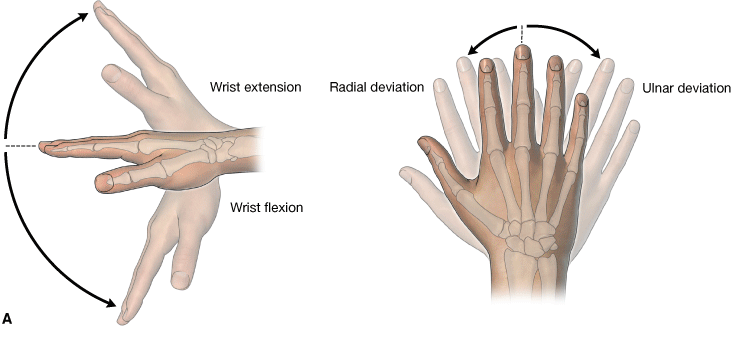
\includegraphics[width=0.5\textwidth]{figures/anatomy/flexexulradev}  %<--but is not needed.
	\caption{Flexion, extension and radial and ulnar deviation of the hand. Modified from \cite{zezo2016}}
	\label{fig:wristMove}
\end{figure}

Several more muscles in addition to those responsible for ulnar and radial deviation are involved with the flexion and extension of the wrist. Like the other muscles, the flexor and extensor muscles also extend through the whole forearm from the distal part of humerus and proximal parts of radius and ulnar to the metacarpal bones in the wrist. Many of these muscles are included in movements of both radial/ulnar deviation and flexion/extension, though flexion/extension have one muscle who is only used for flexion at the wrist, the palmaris longus muscle. This can be explained as more force is usually needed in flexion at the wrist than in extension or radial/ulnar deviation.\\
Though several of the same muscles are included in both types of movement, studies have shown that it is possible to differentiate between recorded EMG signals from these muscles when performing radial/ulnar deviation and flexion/extension at the wrist. \cite{hahne2014} In \figref{fig:ALL_THE_MUSCLES} the muscles in the forearm both involved with extension/flexion and radial/ulnar deviation is marked with boxes around the name of the muscles. 

\begin{figure}[H]
	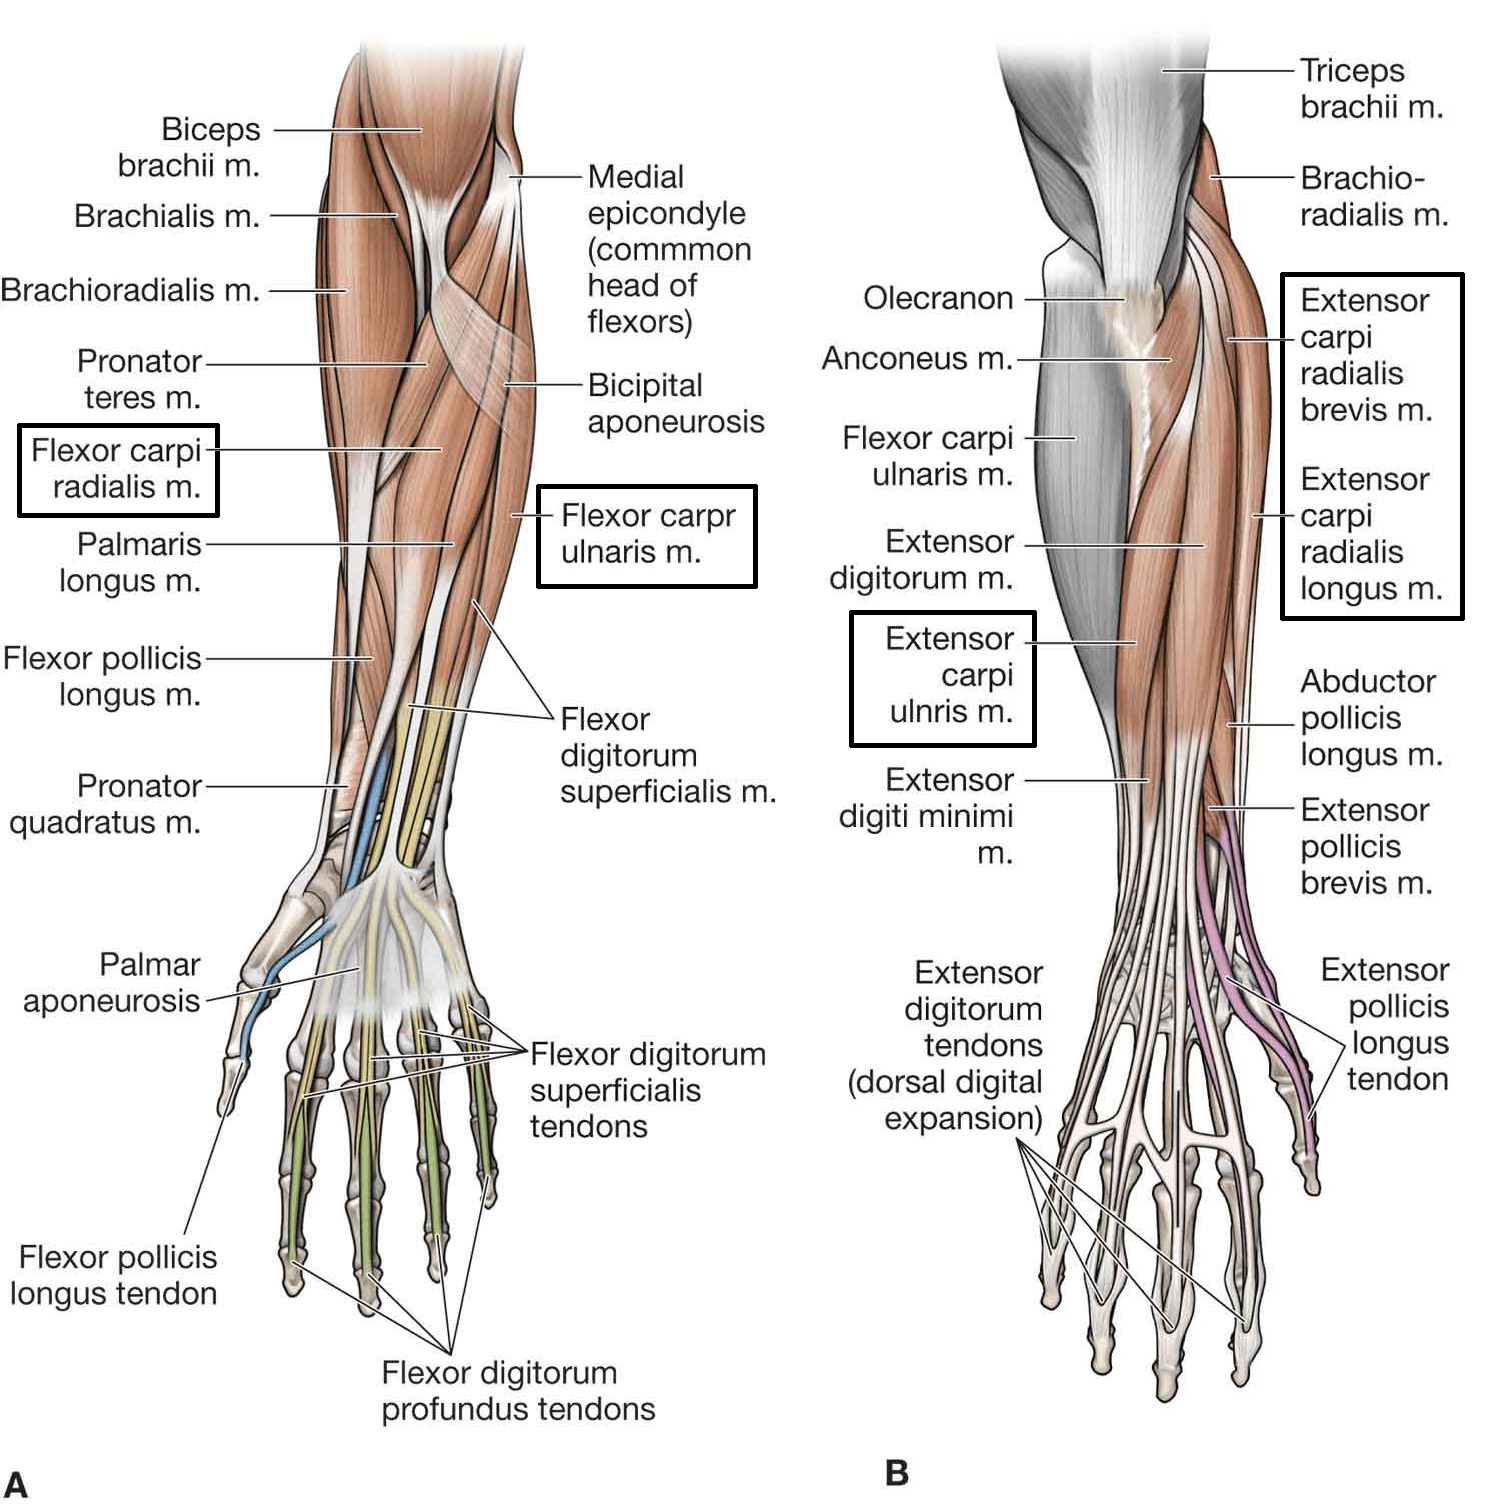
\includegraphics[width=0.7\textwidth]{figures/anatomy/all_the_muscles}  %<--but is not needed.
	\caption{\textbf{A)} anterior view of lower muscles. \textbf{B)} posterior view of lower muscles. The muscle names in the boxes are muscles which are included in both extension/flexion and ulnar/radial deviation at the wrist. Modified from \cite{zezo2016}.}
	\label{fig:ALL_THE_MUSCLES}  %<--give the figure a label, so you can reference!
\end{figure}

%Muscles involved with pronation of the wrist includes the pronator quadratus and pronator teres muscles. The pronator quadratus muscle is located near the wrist and is fixated on the distal portions of both ulna and radius, from where is forms a wide band across the gap of the two bones. The pronator teres is located near the elbow, where it originates  from the medial distal part of humerus and the medial lateral part of ulna, to reach across the anterior part of the forearm and fixate to the midlateral surface of radius. 
%There is only one muscle involved in the process of supination of the forearm, the supinator. The supinator muscle sits opposite the pronator teres muscle near the elbow, where it originates from the lateral distal part of humerus and the lateral proximal part of ulna and fixate on the anterolateral surface of radius. 
%These three are the only muscles responsible for pronation and supination of the forearm. Therein exists a problem in detecting viable EMG signals to properly detect pronation and supination gestures, since the muscles involved does not extend through the forearm as most other muscles in the forearm.

%Extension and flexion of the fingers include most of the muscles in the lower arm. Most of these muscles extend throughout the whole forearm as most of them originates from the lateral surfaces of humerus or the proximal portions of ulna and radius, and extends towards the wrist and fingers to fixate on the metacarpal bones in the wrist and through tendons fixate on the different phalanges bones of the fingers and thumb. See FIGURE \ref{fig:wrist} and \ref{fig:wristFingers} for a detailed overview of each muscles origin, insertion and action it performs. 
%
%\begin{figure}[H]
%	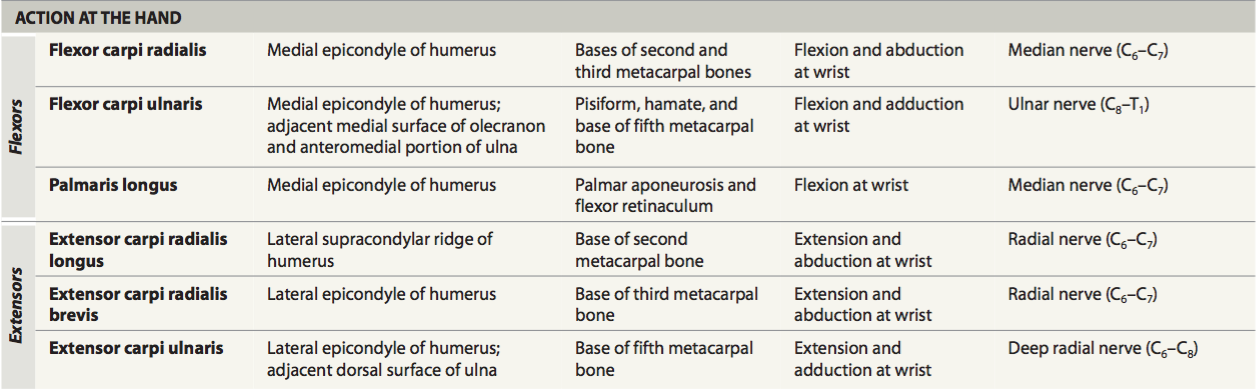
\includegraphics[width=.4\textwidth]{figures/Anatomy/wrist}  %<--but is not needed.
%	\caption{Table of the muscles in the forearm involved with movements of the wrist. \cite{martini}}
%	\label{fig:wrist}  %<--give the figure a label, so you can reference!
%\end{figure}
%
%\begin{figure}[H]                    
%	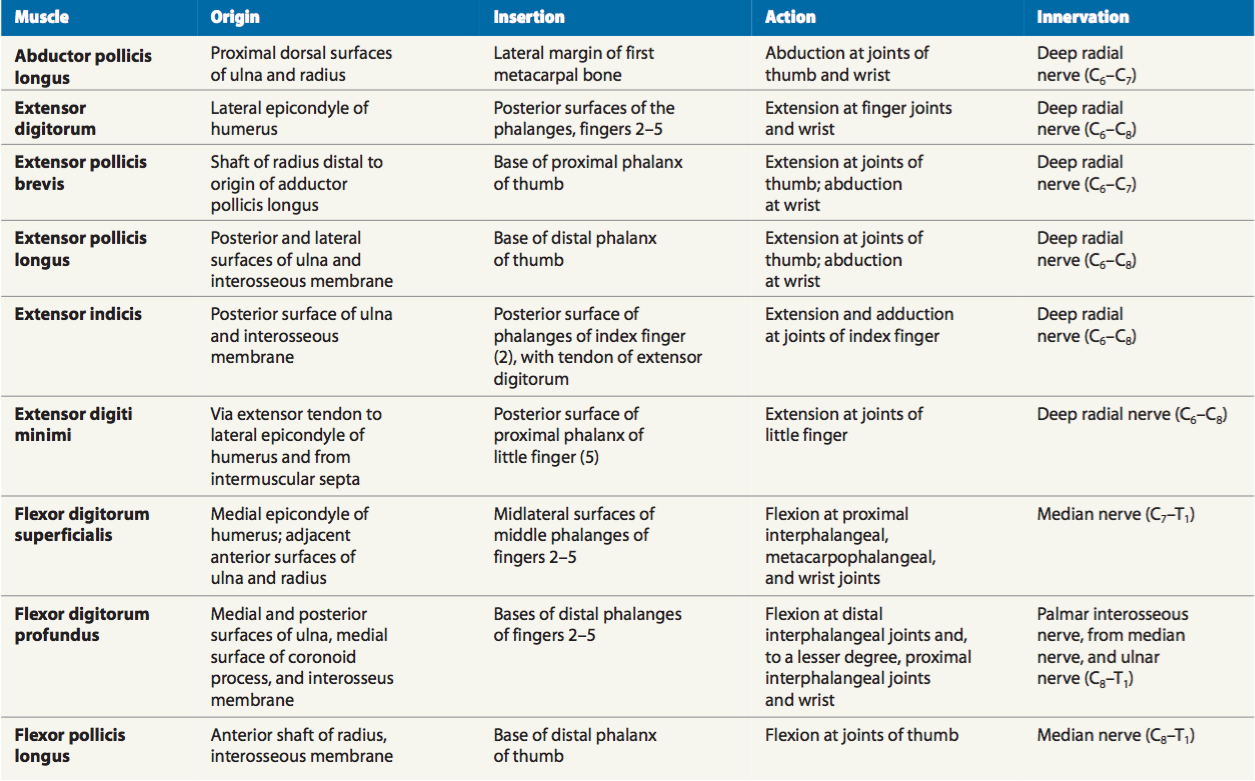
\includegraphics[width=.4\textwidth]{figures/Anatomy/wristFingers}  %<--but is not needed.
%	\caption{Tabel of muscles in the forearm involved with movements of the wrist and fingers. \cite{martini}}
%	\label{fig:wristFingers}  %<--give the figure a label, so you can reference!
%\end{figure}



%abductor pollicis longus
%extensor pollicis longus
%extensor pollicis brevis
%extensor indicis
%supinator
%anconeus
%extensor digitorum
%extensor digiti minimi
%pronator quadratus
%flexor digitorum superficialis
%brachialis
%flexor pollicis longus
%flexor digitorum profundus
%brachioradialis
%flexor carpi ulnaris
%pronator teres
%extensor carpi ulnaris
%extensor carpi radialis brevis
%extensor carpi radialis longus
%palmaris longus
%flexor carpi radialis




%tail


\section{Origin of electromyography} \label{sec:physiology}
This project will use EMG to map the hand gestures mentioned in the previous section. In this section it will be described how the EMG signal is generated.% and which problems that can occur in detecting it. 

The electric potential detected with electromyography is an action potential causing the muscle to contract. Certain mechanisms are involved for this to happen. The motor unit of the muscle needs to be activated alongside with its associated alpha motor system, which is the lower motor neuron, its axon, and the muscle fibres the motor unit innervates. The muscle fibre is an excitable cell with a resting potential of between -90mV and -70mV. A threshold of approximately -55mV needs to be reached for an action potential to be generated, this is visualised in \figref{fig:action_potential}. The sarcolemma, the membrane covering the muscle fibres, has sodium and potassium ion channels that maintains the resting potential, depolarize the muscle fibre if the threshold is exceeded or repolarize the muscle fibre. \cite{cram2012}


\begin{figure}[H]
	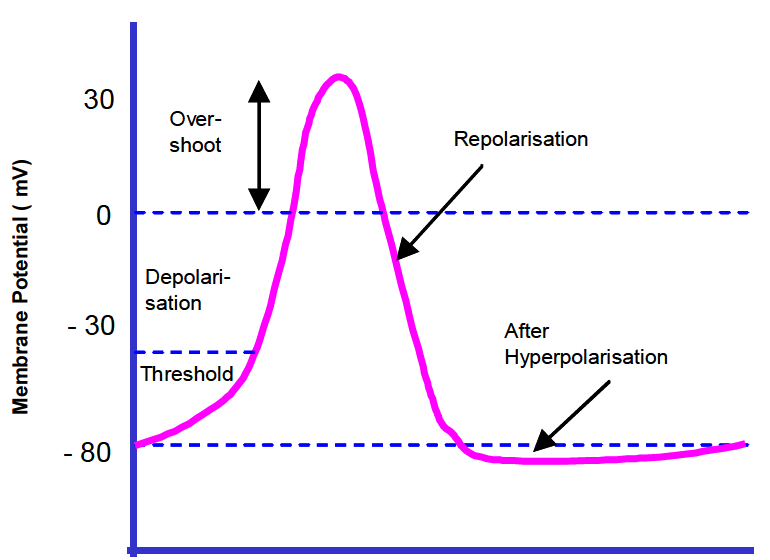
\includegraphics[width=0.5\textwidth]{figures/Anatomy/action_potential}  %<--but is not needed.
	\caption{Illustration of the action potential exceeding the threshold for it to be generated and the following depolarization and repolarization. \cite{konrad2005}}
	\label{fig:action_potential}  %<--give the figure a label, so you can reference!
\end{figure}

The lower motor axon is branching out so that it can attach to the muscle fibre at the motor end-plate and create neuromuscular synapses. The action potential traveling down the axon reaches the synapses and releases Acetylcholine (ACh). ACh raises the permeability of the cell membrane where sodium ions influx and causes the membrane to depolarize. Calcium ions are released and binds with troponin and expose the active sites on the thin filaments which allows the muscle to contract. The action potential travels along the whole muscle fibre through t-tubuluses, as depicted in \figref{fig:EMG_generation}. This happens in both directions from the motor end-plate to the tendinous attachment. When the peak of the depolarization of about 30mV is reached a rapid efflux of potassium ions causes the muscle fibre to repolarize and reach its resting potential again. \cite{cram2012}

\begin{figure}[H]
	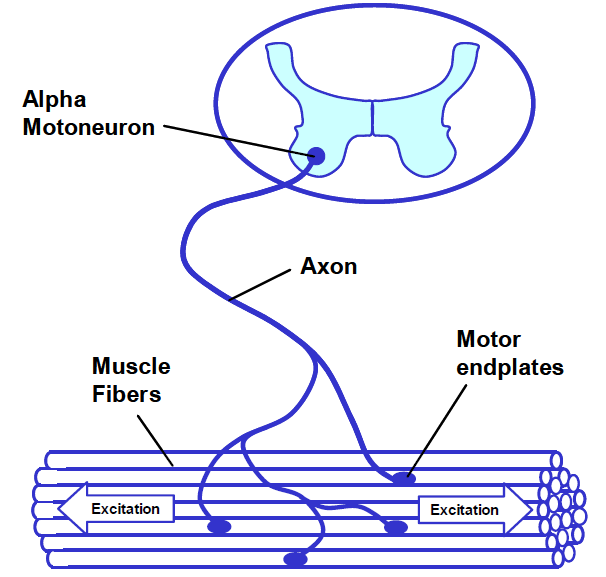
\includegraphics[width=0.4\textwidth]{figures/Anatomy/EMG_generation}  %<--but is not needed.
	\caption{Illustration of the action potential exciting the muscle fibre, which causes the release of calcium ions and the muscle to contract. \cite{konrad2005}}
	\label{fig:EMG_generation}  %<--give the figure a label, so you can reference!
\end{figure}

Depending on the force that needs to be applied for a given task more or less motor units are activated and therefore more or less muscle fibres are contracted. The bigger the force the more motor units are activated. Furthermore, the number of muscle fibres per motor unit varies between muscles in the human anatomy. The finer the movement the higher the innervation, e.g. the lower arm muscles have a higher innervation than those in the quadriceps. \cite{cram2012}

\subsection{EMG states}
Motor unit action potential (MUAP) can be easily decribed as the addition of the action potentials emerging from the muscle fibers comprising the motor unit. The EMG signal is the result of the inclusion of different MUAP.

 %JACOB COMENT:and can be divided into two main states, the transient state and the steady state.Before write is true for  ramp and hold contraction not for every contraction (training protocol related)
 The transient state is related to the beginning phase of the muscle contraction, while the steady state is the stable phase of the muscle contraction when a constant position is held. \cite{mobarak2014}

Although the steady state only contains a short temporal structure of the patterns involved in the contraction of the muscle \cite{mobarak}, studies has shown that it is possible to achieve online continuous control using steady-state EMG signals. A study by Englehart et al. \cite{} demonstrated that steady-state data classified more precisely than transient state data. This could be due to the fact that a larger amount of meaningful data is contained in this muscle contraction phase \cite{mobarak} For the training of the control system  in this project the steady signal will then be used. %However there are still limitations due the fact that the classifier can not deal with the transient EMG signals. Some clinical applications that combine both data have shown an increase in the recognition system.  

%the extraocular muscle has the highest innervation of 3:1 and the gastrocnemius muscles has one of 2000:1. \cite{cram2012}

%(Something about how the innervation is in certain muscles of the forearm. Also argue that humans can perform more dexterous movement when the ratio of muscle fibers to motor units is low) (maybe around 100:1)

%(something about how the EMG signal is affected when the limb is positioned differently)
% following section move to the "conclusion of the background" section
%As mentioned this project focuses on the mapping of different hand gestures. This mapping relies on that the generated EMG from the different hand gestures are differentiable. For a prosthetic user a good performing prosthesis must perform hand gestures as well in an elevated limb position as in a seated position to be able to support the user in daily tasks, e. g. taking a cup from a cupboard and pouring water into the cup. However, changes in the EMG occurs when performing the same hand gestures in different limb positions. These signal alternations can occur for different reasons. Changing the limb position can lengthen the muscles and result in a change in the signal source relative to the electrode from which the EMG signal is obtained, and even the lengthening of the muscles itself due to changing limb position will alter the EMG activity caused by a degree of overlap of the thick and thin filaments. Other findings has shown that the activity of certain muscles' is depending on angles of joints besides those primarily actuating the contraction of these muscles. \cite{Fougner2011} Thus, this limb position effect must be seen as an important aspect to take into consideration in the mapping of hand gestures to control a prosthesis for the user to receive a good performing support device. 
\section{Some stuff and such stuff and other stuff too}

The following section will contain an explanation of the two main components when acquiring EMG signals, including different electrode designs and the most common preprocessing methods used in EMG acquisition.

\subsection{Electrode function and selection}

When performing EMG the electrodes act as a transducer by converting the differences in ion distribution on the skin surface caused by ion exchange under muscle activity, into an electric current. Electrodes used to aquire EMG signals comes both with and without gel covered surfaces, where the the Myo Band employs dry electrodes. Using dry electrodes will often be more practical in use, while the gel covered electrodes will aquire more exact readings of the signals. \cite{lee2008 , cram2012}

The most commonly used electrodes for EMG are made of disposable silver-impregnated plastic, and in order to keep the electric potential on the skin surface stable and reduce impedance between the surfaces, they are often covered in a silver chloride gel. Using dry electrodes will result in  a higher surface impedance, which means that the signal contains more noise compared to a gel covered electrode.\cite{cram2012}

\subsection{Preprocessing of EMG}

In order to achieve a higher signal to noise ratio (SNR) it is common practice to implement some preprocessing methods, including input impedance, differential amplification and filtering. The raw EMG signals has to be preprocessed due to them sensible to noise elements from the surroundings, since the range of the signal is in the order of millivolts to microvolts.\cite{cram2012}

Input impedance is determined by a simple rule in order to avoid defeating the common mode rejection of the EMG amplifier. The rule states that the input impedance of the EMG amplifier has to be between $10$ and $100$ times higher than the impedance of the skin-electrode interface.\cite{cram2012}

Differential amplification is used in EMG in order to amplify the original signal and remove common signals from two or more electrodes, in order to avoid common noise from more electrodes in the amplified signal. The amplifier has a build in gain as well, which determines the final strength of the signal, and both of these features are implemented in order to avoid the SNR.\cite{cram2012}

Basic filtering should be implemented in order to avoid electrical noise (50 or 60 Hz). This filter would be implemented as a notch filter, in order to reject the electrical noise and achieve a higher SNR. Furthermore the filtering should include a bandpass filter with a bandwith chosen depending on where the EMG is performed. This is done in order to make sure the final signal doesn't contain irrelevant high and low frequencies.\cite{cram2012}
\section{Instrumentation} \label{sec:myoband}
	% former Myo armband -section
%What does the band consist of?
%Electrodes, gyroscope and accelerometer
%Build-in filters and stuff like that?
%Sampling frequency

%head
The following section will contain a presentation of the Myo armband from Thalmic Labs, which will be used for data acquisition in this study and an explanation of acquiring EMG signals using surface electrodes.

\subsection{Myo armband}

The Myo armband is a device developed by Thalmic Labs capable of identifying hand gestures and arm movements in order to interact and control different electronic devices. The system can be used with software provided by Thalmic Labs to control a limited range of devices using the data from the armband.
%However, standard use of the system does not provide use of the raw data, which is necessary for this project. The system does however allow data to be extracted from the armband, with without involving the software from Thalmic Labs. This enables to acquire data to process in Matlab. 
The Myo armband is illustrated in \figref{fig:armband}. 

\begin{figure}[H]                    
	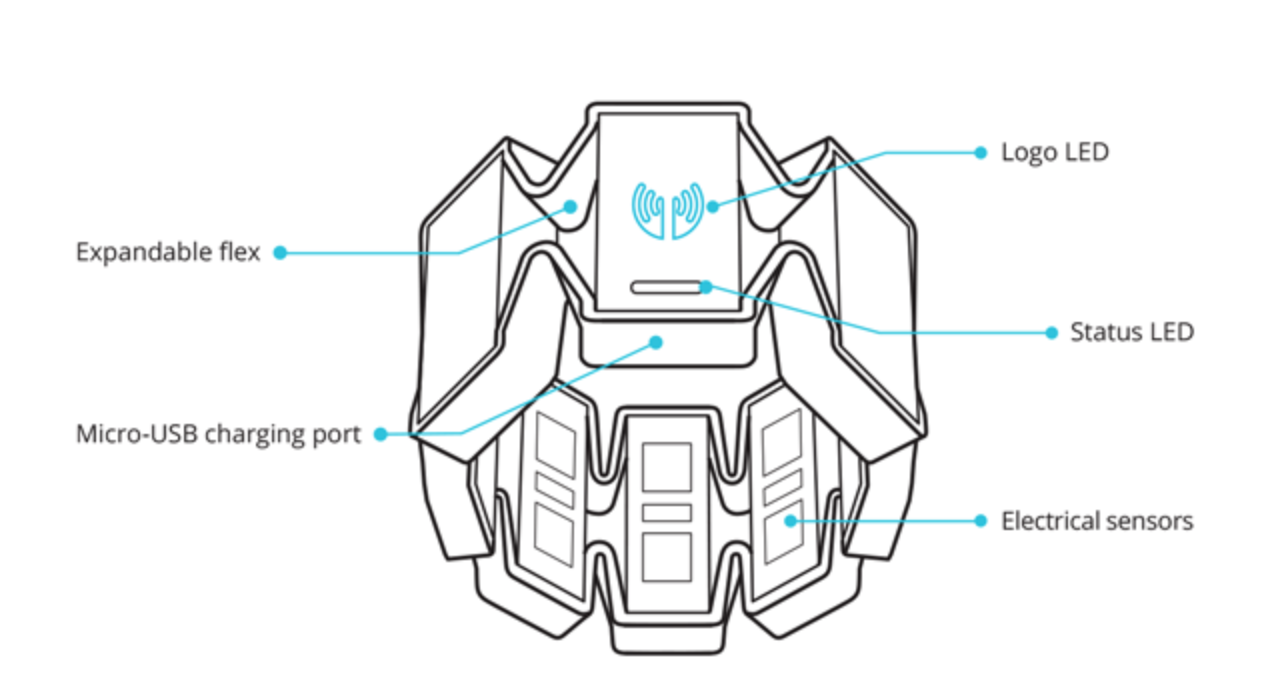
\includegraphics[width=.5\textwidth]{figures/myob/armband}  %<--but is not needed.
	\caption{Main components of the Myo armband. \textbf{SOURCE}}
	\label{fig:armband}  %<--give the figure a label, so you can reference!
\end{figure}


%The main components of the Myo armband illustrated in the figure \ref{fig:armband} are:
%\begin{itemize}
%\item The logo LED gives information about the sync state. The LED is solid when you perform the Sync Gesture successfully and
%the Myo armband is synced to your arm. The LED pulses when the armband is not synced.
%\item The status LED shows the state of the Myo armband. When it lights up in blue once the Myo armband is connected to a device. 
%\item The USB charging port allows to charge the Myo armband battery. 
%\end{itemize}
%The systems counts with sizing clips, these small pieces give a tighter grip which is more appropriated for smaller arms.

The Myo armband has eight medical grade stainless steel surface EMG sensors. %responsible of recognizing each gesture. 
These electrodes are dry and therefore not covered in silver chloride gel to reduce impedance between the electrode and skin. However, it has been shown by Mendez et al. \cite{Mendez2017} that the EMG recorded with the Myo armband is a suitable acquisition system for mapping hand gestures compared to conventional EMG acquisition. The only mapping method used in that study was linear discriminant analysis, and it is noted that other mapping methods should be investigated to further validate the quality of mapping the EMG obtained by the Myo armband. The Myo armband is sampling sEMG data at a sample rate of 200 Hz. A low sample rate could result in problems of aliasing later on in the data processing, since the range of the sEMG signal is 10-500 Hz. \cite{cram2012} 

In addition, it has a nine axis inertial measurement unit (IMU) which enable the detection of arm movement. An IMU is an electronic device that provides information concerning position and orientation for navigation and stabilization purposes. The IMU's in the Myo armband comprises a three axis accelerometer, a three axis gyroscope and a three axis magnetometer. The accelerometer measures the physical acceleration experienced by an object, where the object in this case is the body part where the Myo armband is placed. 
%It gives information about the acceleration experienced relative to free fall and expresses this in g-force. One g-force being when the accelerometer is at rest on the Earth's surface. That is since all points on the surface of the Earth is accelerating upwards relative to an object in free fall near the surface. For the g-force to change from one g-force the accelerometer must be exposed to motion. 
The gyroscope has the property of measuring angluar velocity. The magnetometer has the property of a compass, measuring the earth's magnetic field. This enables the armband to provide data on orientation. IMU data is sampled at a sample rate of 50 Hz. The Myo armband communicates through Bluetooth 4.0 to a computer.
%(something about the actual data the myoband provides and how many axes a magnometer actually has). \textbf{SOURCE}
%\textbf{more text on the data types we are going to get from the IMU's} 
% ... (It is equipped with an ARM Cortex-M4 microprocessor of low energy consumption.)

%\begin{figure}[H]                    
%	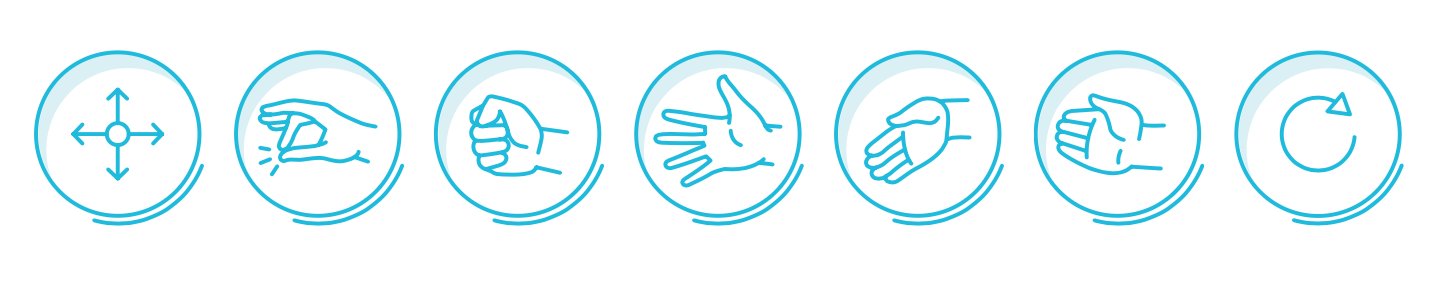
\includegraphics[width=.5\textwidth]{figures/myob/gestures}  %<--but is not needed.
%	\caption{Hand gestures and movements detected by the Myo armband using its own interface from Thalmic Labs. SOURCE}
%	\label{fig:gestures}  %<--give the figure a label, so you can reference!
%\end{figure}
%It offers five pre-defined gestures as showed in the figure \ref{fig:gestures}, it provides haptic feedback through short, medium or long vibrations to correct moves or activate the system.

%JACOVB COMENT:sample rate high enough


%This means that many high-frequencies of the sEMG signal will not be recorded, and aliasing could have an influence on the recorded signals due to not respecting the Nyquist Law of sample rate. 
%Thus, the Myo band arm supplies two kinds of data, the IMU data and EMG data. %which is spatial and gestural. 
%The IMU data add information about the orientation and movement of the user's arm. This information is provided through the accelerometer and the gyroscope. EMG recordings gives information about the users hand gestures. The recorded signals can be send to other devices using Bluetooth 4.0.


%/begin{figure}
%poner imagen del los gestos%
%/end{figure}

%How does it communicate with the computer?
%Connection
%Programs that can be used to interface with the arm
%What kind of data will be received from the myo band?


%it connecrs to a PC or tablet via bluetooth Low Energy and allows both raw data streaming and the use of a proprietary library for gesture recognition.The signal processing is performed on the host platform and the used algorithms are not documented (poner de otra manera)



\section{JACO2 robotic arm}

In this section a briefly description of the JACO$^2$ robotic arm will be given. It is a 6 DOF robotic arm  with a three fingered hand developed by Kinova Robotics. It is lightweight $\left( 4.4 kg\right)$, which makes this machine specially usable in assistive and collaborative applications. It is designed to help people with upper body disabilities in order to gain more autonomy in ordinary daily tasks.\\

\begin{figure}[H]                    
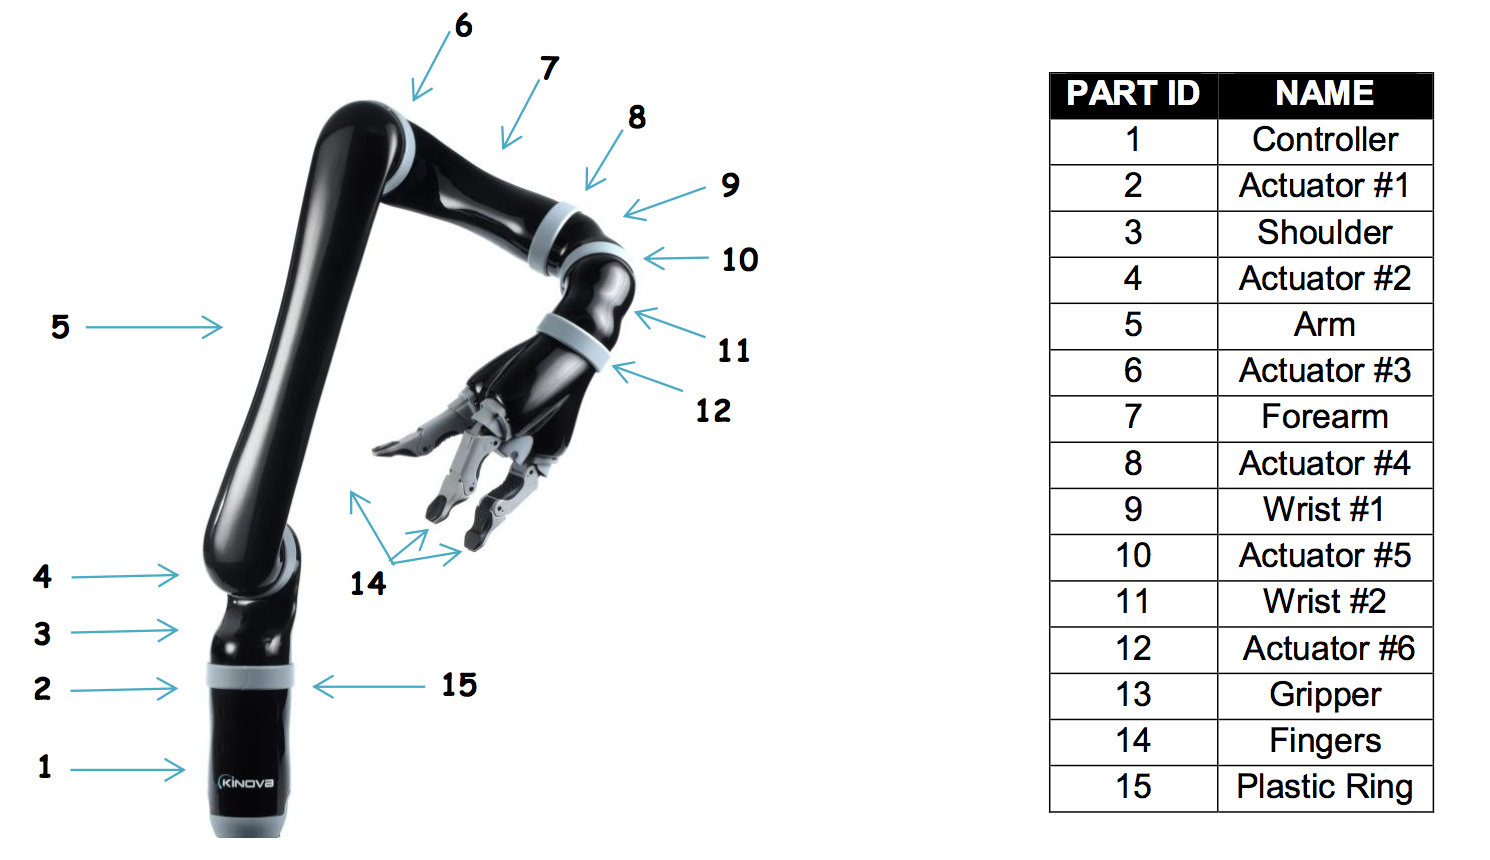
\includegraphics[width=.3\textwidth]{figures/Jaco/roboticarm}  %<--but is not needed.
\caption{6 DOF JACO$^2$ robotic arm from Kinova Robotics. \cite{kinova2017}}
\label{fig:roboticarm}  %<--give the figure a label, so you can reference!
\end{figure}
\textbf{new more exciting picture of the same thing}

The JACO$^2$ is a serial manipulator, which means that this kind of robotic arm is designed as a series of links connected by motor-actuated joints that extend from a base to an end-effector. Any movement in a joint affects all the following joints and links in the chain. The arm can by default be controlled with the help of a joystick, but it can be programmed in C++ to be controlled by other means, using the software development kit (SDK) provided by the manufacturer.\\

\textbf{include picture of JACO arm with all the names of things on/in it.}

%The control of the JACO$^2$ arm can be Angular and Cartesian. In Angular control each actuator moves separately. Cartesian robots called Gantry robots as well, are mechatronic devices which make linear movements in three axes, perpendicularly oriented to each other. It allows eight movements:
%\begin{itemize}
%\item Three translations
%\item Three rotations of the wrist
%\item Two movements of the fingers $\left( open/close\right) $
%\end{itemize}


\section{Preprocessing of EMG}

%HEAD
Before recorded EMG signals can be utilized in control of prosthetics, the signals must be processed. This section will provide information on preprocessing of the signal with filtering and noise reduction, following with feature extraction.

As mentioned in \secref{sec:myoband} sEMG is in a 10-500 Hz range. Thus it is recommended to implement a bandpass filter from $10$ to $500$ Hz in order to avoid low frequency movement artifacts in the recorded signal. 
%If the EMG is acquired from an area close to the heart, it would be preferable to filter from $100$ Hz in order to avoid recording artifacts from the heart. 
A downside to this bandwidth is that fatigued muscles will fire at a lower rate, which means the performance of the system will be affected when the subject gets tired. \cite{cram2012} %Due to the frequency spectrum of the Myo band, it isn't required to implement a bandpass filter. Instead the signal will be subjected to a highpass filter from $5$ Hz. (The frequency spectrum should be mentioned in the Myo band section and not here I think)

In order to achieve a higher signal to noise ratio (SNR) it is common practice to perform preprocessing of the signal%, including input impedance, differential amplification and filtering. 
The raw EMG signals has to be preprocessed due to them being sensible to noise elements from the surroundings, since the range of the signal is in the order of millivolts to microvolts. To acquire a high SNR, the input impedance of the amplifier has to be between $10$ and $100$ times the impedance at the skin-electrode interface \cite{cram2012}.

%Input impedance is determined by a simple rule in order to avoid defeating the common mode rejection of the EMG amplifier. The rule states that the input impedance of the EMG amplifier has to be between $10$ and $100$ times higher than the impedance of the skin-electrode interface. \cite{cram2012}

Differential amplification is used in EMG in order to amplify the original signal and remove common signals from two or more electrodes, in order to avoid common noise from more electrodes in the amplified signal. The amplifier must have a built in gain as well which determines the final strength of the signal, and both of these features are implemented in order to maximize the SNR. 
%Basic filtering should be implemented in order to avoid electrical noise. 
%This filter would be implemented as a notch filter, in order to reject the electrical noise and achieve a higher SNR. 
%The low-pass filtering will ensure avoiding aliasing in the signal, because is will filter out frequencies higher than the used samplings frequency. The high-pass filter will filter out movement artifact, and thus stabilizing the baseline. \cite{cram2012}

%This is done in order to make sure the final signal does not contain irrelevant high and low frequencies.\cite{cram2012}

%feature extraction follows here as a sbusection
\subsection{Feature extraction}

% Use 'Linear and non linear regression techniques for Simultaneus and prop...' + 'Feature reduction and selection for EMG signal classification'

%HEAD
%The following section will feature feature extracion, 

Following preprocessing of the recorded EMG signal, features can be extracted and used to map different hand gestures. Features are extracted from the signal to represent the signal using fewer data samples. This is also called dimension reduction and result in faster computation times. When analyzing EMG signals there will be three different signal components to be extracted, which are the frequency and time domains, as well as the time-scale representation. Frequency domain features require a Fourier transformation of the signal, which requires more processing than the direct extraction of time domain features. \cite{phiny2012}
%In order to extract the features which can be used to differ between the movements performed by the wearer, different features can  extraction can be implemented. In addition to highlighting important features within the signal, the implementation of feature extraction will be useful when it comes to removing unwanted signal features caused by noise sources such as the powergrid and movement of the electrodes. \cite{phiny2012}

The time domain features are extracted directly from the EMG signal, and these feature extraction methods are often used both for research and practices since they often require very little processing compared to frequency domain features. Time domain features are mainly focused on the amplitude of the signal, which means they have a disadvantage if the signal differs in amplitude due to muscle fatigue. \cite{phiny2012} Different features are visualized in \figref{fig:EMGfeatures}. 

\begin{figure}[H]                    
	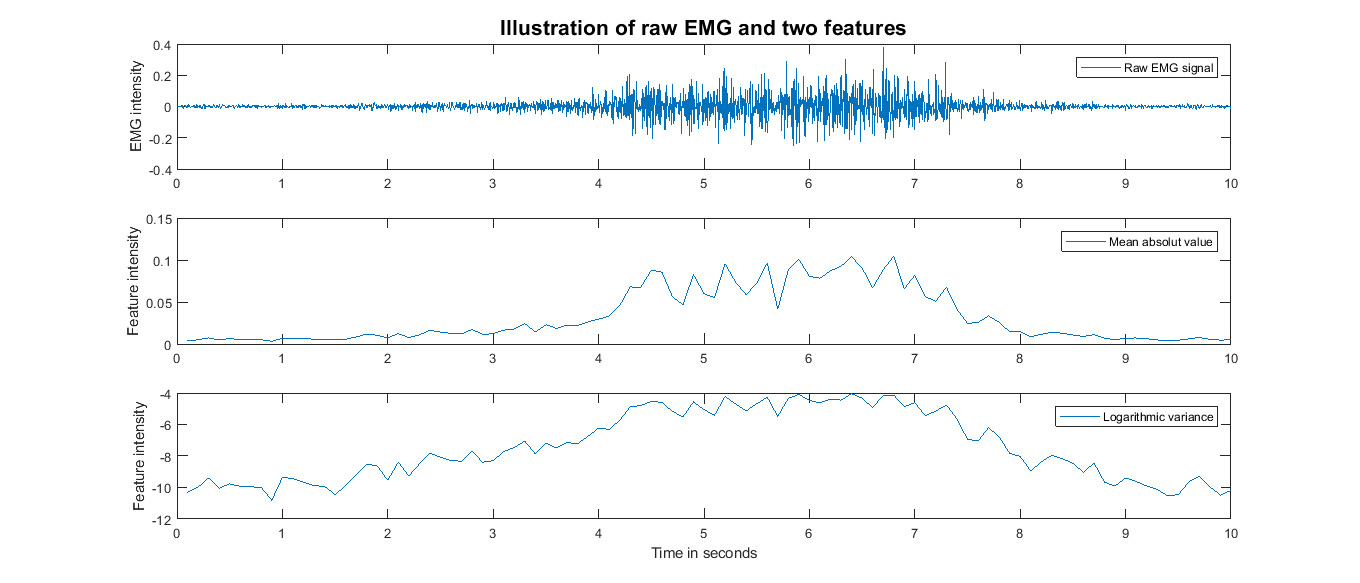
\includegraphics[width=.5\textwidth]{figures/background/EMG_features}  %<--but is not needed.
	\caption{Above a raw EMG signal. Below are different features extracted from the EMG signal presented.}
	\label{fig:EMGfeatures}
\end{figure}

%Based on the study af Hahne et al. \cite{hahne2014}, we will choose logarithmic variance as the feature to be extracted from the recorded EMG signal. Hahne et al. finds that the cross-validation performance improves significantly with the use of linear regression combined with logarithmic variance, compared to combining the linear regression with variance or RMS. \cite{hahne2014}. 

%Choice of feature will be based on previous studies of performance of different extracted features. 
%%, where the method will be chosen based on it's performance in the low frequency area and the processing time for the feature to be extracted. 
%This is a result of the Myo armband limiting the recordable signal to 100 Hz, and the intend of being able to control the JACO arm in real-time, where a long processing time would cause a delay between hand movement and movement of the JACO arm.
%This study will only implement time domain features, due to the low sampling rate of the Myo band, which means that an implementation of frequency domain features will not be useful, as the signal does not contain a lot of information in that domain. The feature chosen in this study will be the logarithmic variance of the signal, based on a previous study by \cite{hahne2014}, where they find that this feature is useful for methods based on the numerical range of the features. \cite{hahne2014} 
\section{Regression methods}

%Linear regression:
	%linear regression (how well the line fits the data can be decided with goodnes of fit or least squares)
	%multiple linear regression
	%principal components regression
	%bayesian linear regression
%non-linear regression:
	%kernel ridge regression
	%gaussian regression 
	

%head
Regression methods are widely used is statistics as a method to determine relationship between variables. It can be used to extract relations to predict future developments or tendencies in a given data set. It is also a commonly used method to evaluate EMG signals to determine different parameters. 
%There exist many regression methods, but overall to classes of methods can be defined; linear and non-linear, some of which will be covered in this section. 

The most basic form of regression is linear regression, which is a test for linear dependency between two variables. In simple linear regression it is investigated how one, dependent variable, is related to another, independent variable. The term \textit{simple} denotes that only two variables are being considered simultaneously. The equation for simple linear regression is: \cite{zar2009}
\begin{equation}
Y_i = \alpha + \beta X_i
\end{equation}

Performing simple linear regression finds the correlation between the tested variables, and is expressed by the correlation coefficient. This coefficient describes how the two variables relate to each other by how the development of one variable is dependent on the the other. Thus a positive correlation represent that a change in one variable will resolve in a similar change in the other variable as well. On the contrary, a negative correlation imply that change in one variable will resolve in an opposite change in the other variable. If no correlation is present between the two variables no change in either variable will resolve in change in the other, and it can therefore be determined that the two variables has no relation to each other. \cite{zar2009}
The simple correlation coefficient is calculated as: \cite{zar2009}
\begin{equation}
r = \frac{\sum xy}{\sqrt{\sum x^{2} \sum y^{2}}}
\end{equation}

Furthermore a coefficient of determination can be calculated to express how much of the variability of the dependent variable is accounted for when regressing upon the independent variable. This coefficient is denoted $r^{2}$ and can be calculated by simply squaring the correlation coefficient ($r$). 
Both $r$ and $r^{2}$ can be used to determine the strength of the relationship between the two tested variables. \cite{zar2009}


%fit of a straight line to best fit several data points. This regression method is widely used in studies where it is used to describe a simple relationship between a dependent and independent factor.

A variant of the linear regression is the multiple linear regression, which can be used in cases where the relationship between three or more variables is wished to be investigated. Here it is considered that one of the variables are dependent on two or more independent variables. 
Multiple linear regression can be used in cases where two or more variables are expected to have a linear correlation to a dependent variable and it is wished to find which of the independent variables who has the biggest influence on the dependent variable, so to say the highest correlation coefficient. 
Since multiple linear regression is based upon simple linear regression, it is modelled after the equation for simple linear regression. However, as $Y$ can be dependent on more than one other variable at times, another can be added to the equation: \cite{zar2009}
\begin{equation}
Y_i = \alpha + \beta_1 X_1i + \beta_2 X_2i + \epsilon_i \ \ \ \ ,
\end{equation}
, where the sum of the error ($\epsilon$) is zero and is assumed to be normally distributed.

When three variables are present in the equation, the visual representation of the regression is in the 3rd dimension, and will no longer be presented as a line in 2D, but as a plane in 3D. Having more than three variables will resolve in a regression in the $m$-dimension, where $m$ is the number of variables. This plane of regression is called the hyperplane. However, regression is not a perfect fit to every sample point, and thus the equation for three or more variables is only complete when the error is also calculated, denotes as $\epsilon$.

There exist ofcourse cases where the relationship between more than three variables is wished to be investigated. In such cases, each new variable can be added to the equation, and the final can be expressed in a summed up equation: \cite{zar2009}
\begin{equation}
Y_j = \alpha + \sum_{i=1}^{m} \beta_j X_ij + \epsilon_j \ \ \ \ ,
\end{equation}
where $m$ is the number of variables.

There exist no limit to the number of variables which can be tested, however there should always be at least two observations more than the number of variables, so that $n \geq m+2$. Otherwise multiple linear regression is not possible. \cite{zar2009}




%one dependent variable and several independent are to be described and a generalization of the relationship between the variables wish to be found. 

%Principal component regression is based on the principal component analysis, where a very large dataset can be compressed into a few of the most important components to further be analyzed upon. This means that in a dataset of many samples, the ones which are the most responsible or most correlated in a meaningful relationship between the dependent and independent variables, can be isolated to best describe which factors have a result on the relationship.







%tail


\urlstyle{same}
\printbibliography
\cleardoublepage

% BILAG
\begin{appendices}
	
\end{appendices}


\end{document}
